% TikZ figure for papers: a small network diagram with positioning, styles and math labels.
\documentclass[tikz,border=4pt]{standalone}
\usetikzlibrary{positioning,arrows.meta}
\begin{document}
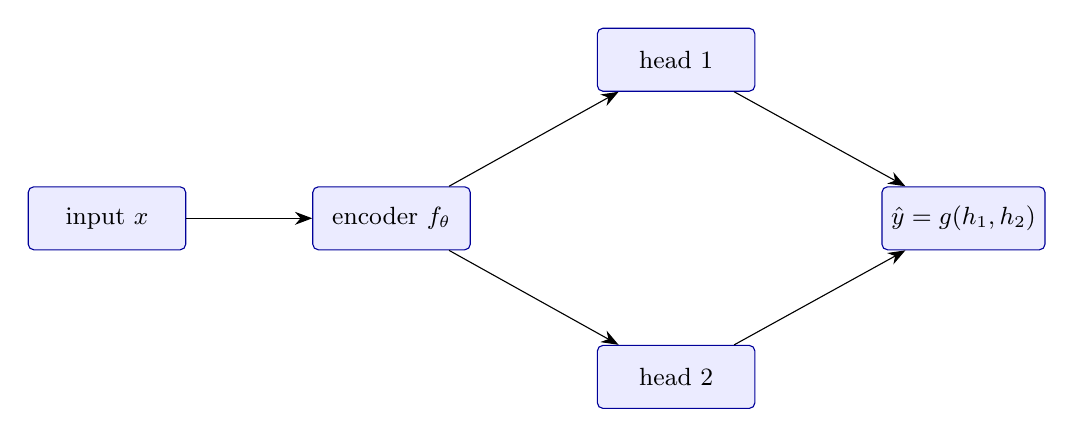
\begin{tikzpicture}[node distance=12mm and 16mm, >={Stealth[length=2.2mm]},
  blk/.style={draw=blue!60!black, fill=blue!8, rounded corners=2pt, minimum width=20mm, minimum height=8mm, font=\small}]
  \node[blk] (x) {input $x$};
  \node[blk, right=of x] (enc) {encoder $f_\theta$};
  \node[blk, above right=of enc] (h1) {head 1};
  \node[blk, below right=of enc] (h2) {head 2};
  \coordinate (m) at (h1.east |- enc);   % level with the encoder, right of the heads: symmetric fan-in
  \node[blk, right=of m] (y) {$\hat y = g(h_1, h_2)$};
  \draw[->] (x) -- (enc);
  \draw[->] (enc) -- (h1); \draw[->] (enc) -- (h2);
  \draw[->] (h1) -- (y); \draw[->] (h2) -- (y);
\end{tikzpicture}
\end{document}
